\section{初识零件图}
图\ref{fig:xiaoluntaotong}被称为零件图。所谓零件图是用于表达零件的图样,它广泛运用于工程技术设计、施工或产品制造,它是制造、加工、测量、检验的依据,是工程界的共同技术语言,是表达和交流技术思想的必备工具,是工程技术部门的一项重要技术文件。掌握零件图的阅读和绘制不仅是构建零件三维模型的基础,也是从事工程设计和技术的工程技术人员所必须具备的基本能力。一张完整的零件图应包括以下几个组成部分:
\begin{itemize}
\item 一组视图
\item 完整的尺寸
\item 技术要求
\item 标题栏
\end{itemize}
\begin{figure}[htbp]
\centering
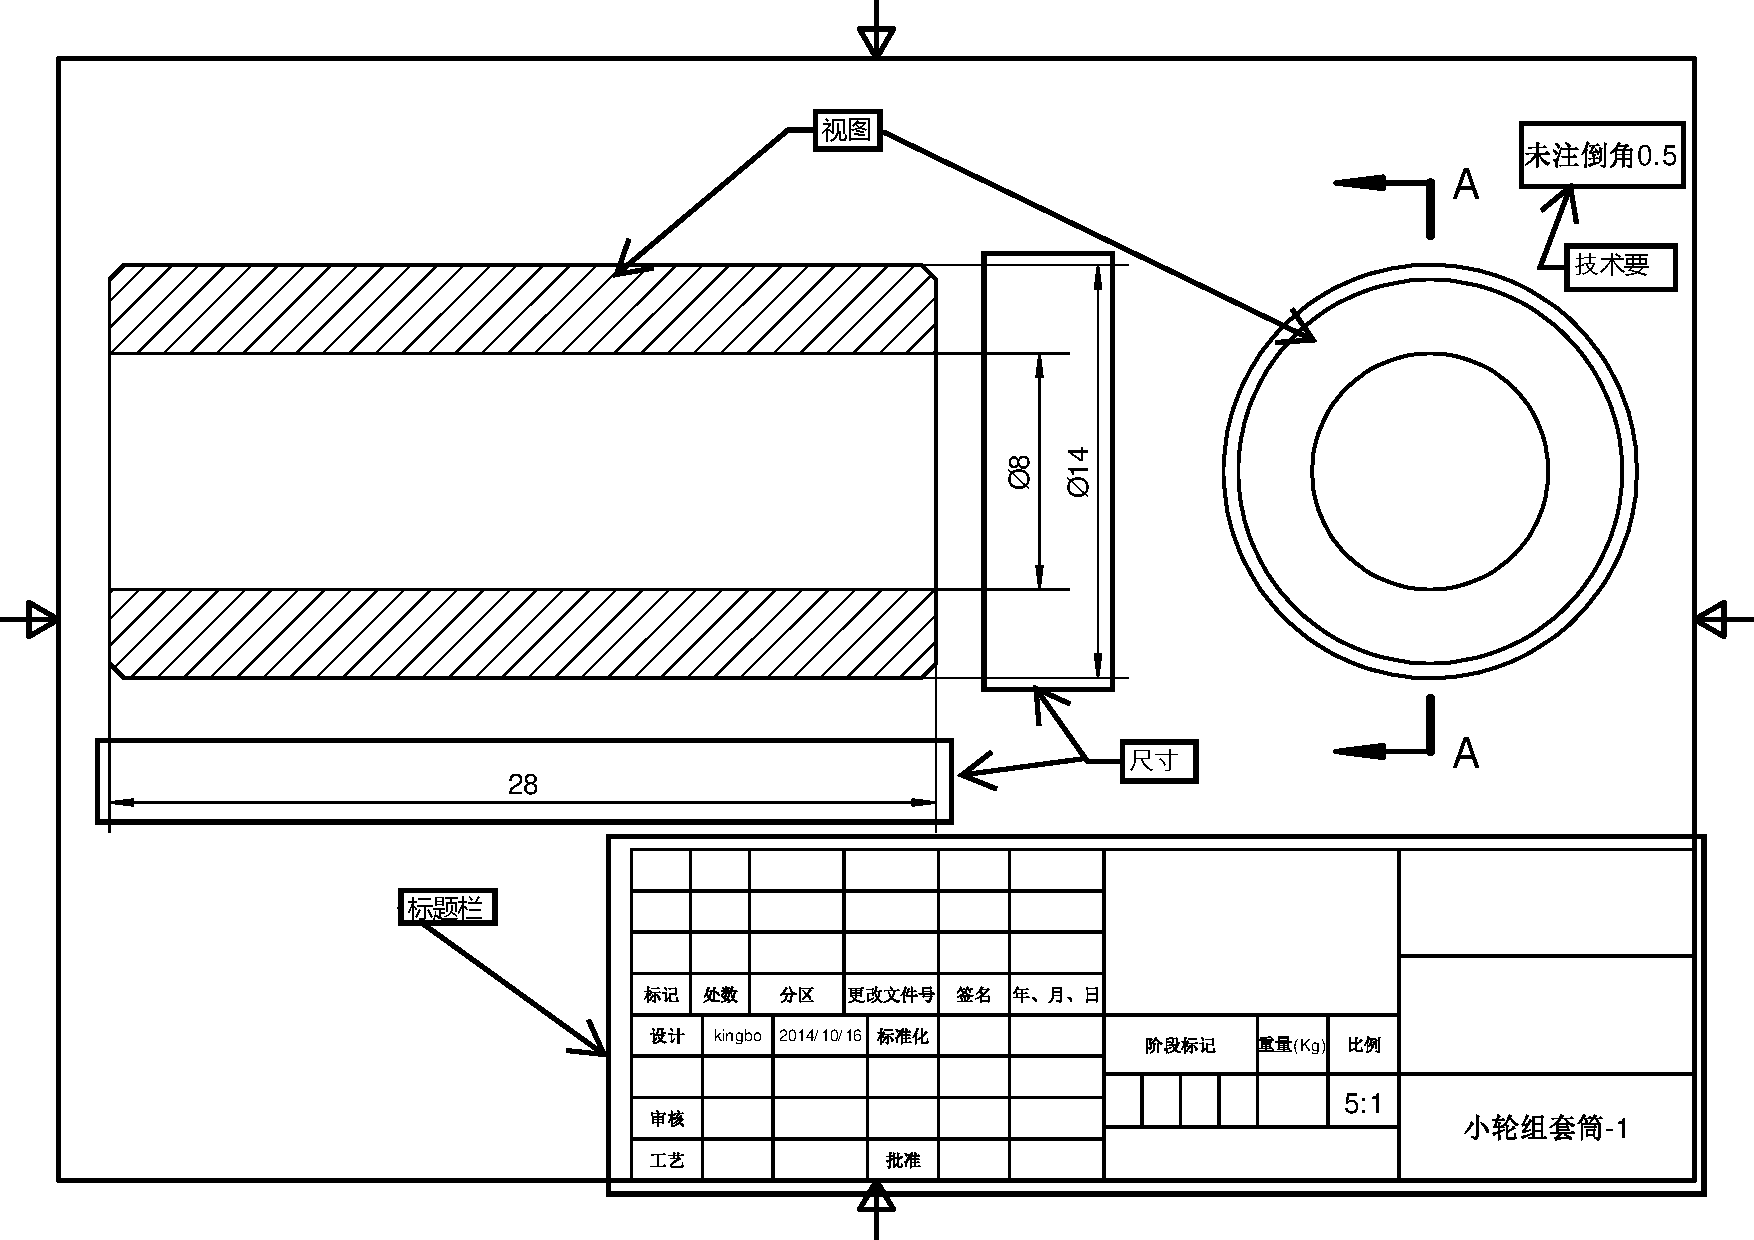
\includegraphics[scale=0.5]{xiaoluntaotong2.pdf}
\caption{零件图组成部分}\label{fig:xiaoluntaotong2}
\end{figure}
图\ref{fig:xiaoluntaotong2}清晰的标识图\ref{fig:xiaoluntaotong}所示零件图的各个组成部分。
\section{理解视图}

\subsection{标题栏}
\subsection{尺寸}

\endinput